% Options for packages loaded elsewhere
\PassOptionsToPackage{unicode,}{hyperref}
\PassOptionsToPackage{hyphens}{url}
\PassOptionsToPackage{dvipsnames,svgnames,x11names}{xcolor}
%
\documentclass[
  titlepage,
  openright,
  DIV=calc,
  toc=listof,
  listof=nochaptergap]{scrbook}
\usepackage{amsmath,amssymb}
\usepackage{setspace}
\usepackage{iftex}
\ifPDFTeX
  \usepackage[T1]{fontenc}
  \usepackage[utf8]{inputenc}
  \usepackage{textcomp} % provide euro and other symbols
\else % if luatex or xetex
  \usepackage{unicode-math} % this also loads fontspec
  \defaultfontfeatures{Scale=MatchLowercase}
  \defaultfontfeatures[\rmfamily]{Ligatures=TeX,Scale=1}
\fi
\usepackage{lmodern}
\ifPDFTeX\else
  % xetex/luatex font selection
\fi
% Use upquote if available, for straight quotes in verbatim environments
\IfFileExists{upquote.sty}{\usepackage{upquote}}{}
\IfFileExists{microtype.sty}{% use microtype if available
  \usepackage[]{microtype}
  \UseMicrotypeSet[protrusion]{basicmath} % disable protrusion for tt fonts
}{}
\makeatletter
\@ifundefined{KOMAClassName}{% if non-KOMA class
  \IfFileExists{parskip.sty}{%
    \usepackage{parskip}
  }{% else
    \setlength{\parindent}{0pt}
    \setlength{\parskip}{6pt plus 2pt minus 1pt}}
}{% if KOMA class
  \KOMAoptions{parskip=half}}
\makeatother
\usepackage{xcolor}
\usepackage[a4paper,bindingoffset=0mm,inner=30mm,outer=30mm,top=30mm,bottom=30mm]{geometry}
\usepackage{color}
\usepackage{fancyvrb}
\newcommand{\VerbBar}{|}
\newcommand{\VERB}{\Verb[commandchars=\\\{\}]}
\DefineVerbatimEnvironment{Highlighting}{Verbatim}{commandchars=\\\{\}}
% Add ',fontsize=\small' for more characters per line
\newenvironment{Shaded}{}{}
\newcommand{\AlertTok}[1]{\textcolor[rgb]{1.00,0.00,0.00}{\textbf{#1}}}
\newcommand{\AnnotationTok}[1]{\textcolor[rgb]{0.38,0.63,0.69}{\textbf{\textit{#1}}}}
\newcommand{\AttributeTok}[1]{\textcolor[rgb]{0.49,0.56,0.16}{#1}}
\newcommand{\BaseNTok}[1]{\textcolor[rgb]{0.25,0.63,0.44}{#1}}
\newcommand{\BuiltInTok}[1]{\textcolor[rgb]{0.00,0.50,0.00}{#1}}
\newcommand{\CharTok}[1]{\textcolor[rgb]{0.25,0.44,0.63}{#1}}
\newcommand{\CommentTok}[1]{\textcolor[rgb]{0.38,0.63,0.69}{\textit{#1}}}
\newcommand{\CommentVarTok}[1]{\textcolor[rgb]{0.38,0.63,0.69}{\textbf{\textit{#1}}}}
\newcommand{\ConstantTok}[1]{\textcolor[rgb]{0.53,0.00,0.00}{#1}}
\newcommand{\ControlFlowTok}[1]{\textcolor[rgb]{0.00,0.44,0.13}{\textbf{#1}}}
\newcommand{\DataTypeTok}[1]{\textcolor[rgb]{0.56,0.13,0.00}{#1}}
\newcommand{\DecValTok}[1]{\textcolor[rgb]{0.25,0.63,0.44}{#1}}
\newcommand{\DocumentationTok}[1]{\textcolor[rgb]{0.73,0.13,0.13}{\textit{#1}}}
\newcommand{\ErrorTok}[1]{\textcolor[rgb]{1.00,0.00,0.00}{\textbf{#1}}}
\newcommand{\ExtensionTok}[1]{#1}
\newcommand{\FloatTok}[1]{\textcolor[rgb]{0.25,0.63,0.44}{#1}}
\newcommand{\FunctionTok}[1]{\textcolor[rgb]{0.02,0.16,0.49}{#1}}
\newcommand{\ImportTok}[1]{\textcolor[rgb]{0.00,0.50,0.00}{\textbf{#1}}}
\newcommand{\InformationTok}[1]{\textcolor[rgb]{0.38,0.63,0.69}{\textbf{\textit{#1}}}}
\newcommand{\KeywordTok}[1]{\textcolor[rgb]{0.00,0.44,0.13}{\textbf{#1}}}
\newcommand{\NormalTok}[1]{#1}
\newcommand{\OperatorTok}[1]{\textcolor[rgb]{0.40,0.40,0.40}{#1}}
\newcommand{\OtherTok}[1]{\textcolor[rgb]{0.00,0.44,0.13}{#1}}
\newcommand{\PreprocessorTok}[1]{\textcolor[rgb]{0.74,0.48,0.00}{#1}}
\newcommand{\RegionMarkerTok}[1]{#1}
\newcommand{\SpecialCharTok}[1]{\textcolor[rgb]{0.25,0.44,0.63}{#1}}
\newcommand{\SpecialStringTok}[1]{\textcolor[rgb]{0.73,0.40,0.53}{#1}}
\newcommand{\StringTok}[1]{\textcolor[rgb]{0.25,0.44,0.63}{#1}}
\newcommand{\VariableTok}[1]{\textcolor[rgb]{0.10,0.09,0.49}{#1}}
\newcommand{\VerbatimStringTok}[1]{\textcolor[rgb]{0.25,0.44,0.63}{#1}}
\newcommand{\WarningTok}[1]{\textcolor[rgb]{0.38,0.63,0.69}{\textbf{\textit{#1}}}}
\usepackage{longtable,booktabs,array}
\usepackage{calc} % for calculating minipage widths
% Correct order of tables after \paragraph or \subparagraph
\usepackage{etoolbox}
\makeatletter
\patchcmd\longtable{\par}{\if@noskipsec\mbox{}\fi\par}{}{}
\makeatother
% Allow footnotes in longtable head/foot
\IfFileExists{footnotehyper.sty}{\usepackage{footnotehyper}}{\usepackage{footnote}}
\makesavenoteenv{longtable}
\usepackage{graphicx}
\makeatletter
\def\maxwidth{\ifdim\Gin@nat@width>\linewidth\linewidth\else\Gin@nat@width\fi}
\def\maxheight{\ifdim\Gin@nat@height>\textheight\textheight\else\Gin@nat@height\fi}
\makeatother
% Scale images if necessary, so that they will not overflow the page
% margins by default, and it is still possible to overwrite the defaults
% using explicit options in \includegraphics[width, height, ...]{}
\setkeys{Gin}{width=\maxwidth,height=\maxheight,keepaspectratio}
% Set default figure placement to htbp
\makeatletter
\def\fps@figure{htbp}
\makeatother
\ifLuaTeX
  \usepackage{luacolor}
  \usepackage[soul]{lua-ul}
\else
  \usepackage{soul}
\fi
\setlength{\emergencystretch}{3em} % prevent overfull lines
\providecommand{\tightlist}{%
  \setlength{\itemsep}{0pt}\setlength{\parskip}{0pt}}
\setcounter{secnumdepth}{-\maxdimen} % remove section numbering
% definitions for citeproc citations
\NewDocumentCommand\citeproctext{}{}
\NewDocumentCommand\citeproc{mm}{%
  \begingroup\def\citeproctext{#2}\cite{#1}\endgroup}
\makeatletter
 % allow citations to break across lines
 \let\@cite@ofmt\@firstofone
 % avoid brackets around text for \cite:
 \def\@biblabel#1{}
 \def\@cite#1#2{{#1\if@tempswa , #2\fi}}
\makeatother
\newlength{\cslhangindent}
\setlength{\cslhangindent}{1.5em}
\newlength{\csllabelwidth}
\setlength{\csllabelwidth}{3em}
\newenvironment{CSLReferences}[2] % #1 hanging-indent, #2 entry-spacing
 {\begin{list}{}{%
  \setlength{\itemindent}{0pt}
  \setlength{\leftmargin}{0pt}
  \setlength{\parsep}{0pt}
  % turn on hanging indent if param 1 is 1
  \ifodd #1
   \setlength{\leftmargin}{\cslhangindent}
   \setlength{\itemindent}{-1\cslhangindent}
  \fi
  % set entry spacing
  \setlength{\itemsep}{#2\baselineskip}}}
 {\end{list}}
\usepackage{calc}
\newcommand{\CSLBlock}[1]{\hfill\break#1\hfill\break}
\newcommand{\CSLLeftMargin}[1]{\parbox[t]{\csllabelwidth}{\strut#1\strut}}
\newcommand{\CSLRightInline}[1]{\parbox[t]{\linewidth - \csllabelwidth}{\strut#1\strut}}
\newcommand{\CSLIndent}[1]{\hspace{\cslhangindent}#1}
\ifLuaTeX
\usepackage[bidi=basic]{babel}
\else
\usepackage[bidi=default]{babel}
\fi
\babelprovide[main,import]{american}
\babelprovide[import]{ngerman}
% get rid of language-specific shorthands (see #6817):
\let\LanguageShortHands\languageshorthands
\def\languageshorthands#1{}
% custom line spacing for quotes
\BeforeBeginEnvironment{quote}{\setstretch{1}}
\AfterEndEnvironment{quote}{\setstretch{1.5}}
\hyphenation
{%
  Hyphenate-me-like-this
  Dontyoueverhyphenateme
}%
% titlepage
\subject{DISS. Nr. 1111\\~\\~\\}
\publishers{A thesis submitted to attain the degree of\\DOCTOR OF SCIENCES\\(Dr. sc.)\\~\\~\\presented by\\~\\Eleanor Roosevelt\\MA, University of Example\\born on 11.10.1884\\~\\~\\accepted on the recommendation of \\~\\Prof. Dr. Anna Hall Roosevelt\\Prof. Dr. Elliott Roosevelt\\~\\2022}
\uppertitleback{Title}
\lowertitleback{\emph{Eleanor Roosevelt} is Fellow at the University of Example.}
\dedication{\emph{For all humants of this world}}
% typesetting options
\clubpenalty=10000
\widowpenalty=10000
\raggedbottom
% number figures consecutively and not chapter by chapter
\usepackage{chngcntr}
\counterwithout{figure}{chapter}
\makeatletter
\@ifpackageloaded{subfig}{}{\usepackage{subfig}}
\@ifpackageloaded{caption}{}{\usepackage{caption}}
\captionsetup[subfloat]{margin=0.5em}
\AtBeginDocument{%
\renewcommand*\figurename{Figure}
\renewcommand*\tablename{Table}
}
\AtBeginDocument{%
\renewcommand*\listfigurename{Figures}
\renewcommand*\listtablename{List of Tables}
}
\newcounter{pandoccrossref@subfigures@footnote@counter}
\newenvironment{pandoccrossrefsubfigures}{%
\setcounter{pandoccrossref@subfigures@footnote@counter}{0}
\begin{figure}\centering%
\gdef\global@pandoccrossref@subfigures@footnotes{}%
\DeclareRobustCommand{\footnote}[1]{\footnotemark%
\stepcounter{pandoccrossref@subfigures@footnote@counter}%
\ifx\global@pandoccrossref@subfigures@footnotes\empty%
\gdef\global@pandoccrossref@subfigures@footnotes{{##1}}%
\else%
\g@addto@macro\global@pandoccrossref@subfigures@footnotes{, {##1}}%
\fi}}%
{\end{figure}%
\addtocounter{footnote}{-\value{pandoccrossref@subfigures@footnote@counter}}
\@for\f:=\global@pandoccrossref@subfigures@footnotes\do{\stepcounter{footnote}\footnotetext{\f}}%
\gdef\global@pandoccrossref@subfigures@footnotes{}}
\@ifpackageloaded{float}{}{\usepackage{float}}
\floatstyle{ruled}
\@ifundefined{c@chapter}{\newfloat{codelisting}{h}{lop}}{\newfloat{codelisting}{h}{lop}[chapter]}
\floatname{codelisting}{Listing}
\newcommand*\listoflistings{\listof{codelisting}{List of Listings}}
\makeatother
\ifLuaTeX
  \usepackage{selnolig}  % disable illegal ligatures
\fi
\IfFileExists{bookmark.sty}{\usepackage{bookmark}}{\usepackage{hyperref}}
\IfFileExists{xurl.sty}{\usepackage{xurl}}{} % add URL line breaks if available
\urlstyle{same}
\hypersetup{
  pdftitle={Title},
  pdfauthor={\href{eleanor.eoosevelt@domain.com}{Eleanor Roosevelt}},
  pdflang={en-US},
  colorlinks=true,
  linkcolor={black},
  filecolor={Maroon},
  citecolor={black},
  urlcolor={black},
  pdfcreator={LaTeX via pandoc}}

\title{Title}
\usepackage{etoolbox}
\makeatletter
\providecommand{\subtitle}[1]{% add subtitle to \maketitle
  \apptocmd{\@title}{\par {\large #1 \par}}{}{}
}
\makeatother
\subtitle{Subtitle}
\author{}
\date{}

\begin{document}
\frontmatter
\maketitle

\chapter*{Abstract}
\begin{spacing}{1.5}
Whereas recognition of the inherent dignity and of the equal and inalienable rights of all members of the human family is the foundation of freedom, justice and peace in the world. Whereas disregard and contempt for human rights have resulted in barbarous acts which have outraged the conscience of mankind, and the advent of a world in which human beings shall enjoy freedom of speech and belief and freedom from fear and want has been proclaimed as the highest aspiration of the common people. Whereas it is essential, if man is not to be compelled to have recourse, as a last resort, to rebellion against tyranny and oppression, that human rights should be protected by the rule of law. Whereas it is essential to promote the development of friendly relations between nations. Whereas the peoples of the United Nations have in the Charter reaffirmed their faith in fundamental human rights, in the dignity and worth of the human person and in the equal rights of men and women and have determined to promote social progress and better standards of life in larger freedom. Whereas Member States have pledged themselves to achieve, in co-operation with the United Nations, the promotion of universal respect for and observance of human rights and fundamental freedoms. Whereas a common understanding of these rights and freedoms is of the greatest importance for the full realization of this pledge. Now, therefore, The General Assembly, proclaims this Universal Declaration of Human Rights as a common standard of achievement for all peoples and all nations, to the end that every individual and every organ of society, keeping this Declaration constantly in mind, shall strive by teaching and education to promote respect for these rights and freedoms and by progressive measures, national and international, to secure their universal and effective recognition and observance, both among the peoples of Member States themselves and among the peoples of territories under their jurisdiction.
\end{spacing}

\begin{otherlanguage}{german}
\chapter*{Zusammenfassung}
\begin{spacing}{1.5}
Die Anerkennung der angeborenen Würde und der gleichen und unveräußerlichen Rechte aller Mitglieder der Menschheitsfamilie ist die Grundlage für Freiheit, Gerechtigkeit und Frieden in der Welt. Die Missachtung und Verachtung der Menschenrechte hat zu barbarischen Taten geführt, die das Gewissen der Menschheit erzürnt haben, und das Streben nach einer Welt, in der die Menschen Rede- und Glaubensfreiheit sowie Freiheit von Furcht und Not genießen, wurde als höchstes Ziel des einfachen Volkes verkündet. Damit der Mensch nicht gezwungen ist, sich als letztes Mittel gegen Tyrannei und Unterdrückung aufzulehnen, ist es unerlässlich, dass die Menschenrechte durch die Rechtsstaatlichkeit geschützt werden. Es ist wichtig, die Entwicklung freundschaftlicher Beziehungen zwischen den Nationen zu fördern. Die Völker der Vereinten Nationen haben in der Charta ihren Glauben an die grundlegenden Menschenrechte, an die Würde und den Wert der menschlichen Person und an die Gleichberechtigung von Männern und Frauen bekräftigt und sind entschlossen, den sozialen Fortschritt und einen besseren Lebensstandard in größerer Freiheit zu fördern. Die Mitgliedstaaten haben sich verpflichtet, in Zusammenarbeit mit den Vereinten Nationen die weltweite Achtung und Einhaltung der Menschenrechte und Grundfreiheiten zu fördern. Ein gemeinsames Verständnis dieser Rechte und Freiheiten ist für die vollständige Verwirklichung dieses Versprechens von größter Bedeutung. Die Generalversammlung verkündet daher diese Allgemeine Erklärung der Menschenrechte als gemeinsamen Maßstab für alle Völker und Nationen, damit jeder Einzelne und jedes Organ der Gesellschaft, die sich diese Erklärung ständig vor Augen halten, sich bemühen, durch Unterricht und Erziehung die Achtung vor diesen Rechten und Freiheiten zu fördern und durch fortschreitende Maßnahmen auf nationaler und internationaler Ebene ihre allgemeine und wirksame Anerkennung und Einhaltung sowohl unter den Völkern der Mitgliedstaaten selbst als auch unter den Völkern der ihrer Hoheitsgewalt unterstehenden Gebiete sicherzustellen.
\end{spacing}
\end{otherlanguage}

\renewcommand*\contentsname{Contents}
{
\hypersetup{linkcolor=}
\setcounter{tocdepth}{2}
\tableofcontents
}
\setstretch{1.5}
\mainmatter
\chapter{Introduction}\label{sec:introduction}

All human beings are born free and equal in dignity and rights. All
human beings are born free and equal in dignity and rights. All human
beings are born free and equal in dignity and rights. All human beings
are born free and equal in dignity and rights.

\section{Heading 2}\label{heading-2}

All human beings are born free and equal in dignity and rights. All
human beings are born free and equal in dignity and rights. All human
beings are born free and equal in dignity and rights. All human beings
are born free and equal in dignity and rights.

\subsection{Heading 3}\label{heading-3}

All human beings are born free and equal in dignity and rights. All
human beings are born free and equal in dignity and rights. All human
beings are born free and equal in dignity and rights. All human beings
are born free and equal in dignity and rights.

\subsubsection{Heading 4}\label{heading-4}

All human beings are born free and equal in dignity and rights. All
human beings are born free and equal in dignity and rights. All human
beings are born free and equal in dignity and rights. All human beings
are born free and equal in dignity and rights.

\section{Bold}\label{bold}

\textbf{All human beings are born free and equal in dignity and rights.}
All human beings are born free and equal in dignity and rights. All
human beings are born free and equal in dignity and rights. All human
beings are born free and equal in dignity and rights.

\section{Italic}\label{italic}

\emph{All human beings are born free and equal in dignity and rights.}
All human beings are born free and equal in dignity and rights. All
human beings are born free and equal in dignity and rights. All human
beings are born free and equal in dignity and rights.

\section{Bold and italic}\label{bold-and-italic}

\textbf{\emph{All human beings are born free and equal in dignity and
rights.}} All human beings are born free and equal in dignity and
rights. All human beings are born free and equal in dignity and rights.
All human beings are born free and equal in dignity and rights.

\section{Struck through}\label{struck-through}

\st{All human beings are born free and equal in dignity and rights.} All
human beings are born free and equal in dignity and rights. All human
beings are born free and equal in dignity and rights. All human beings
are born free and equal in dignity and rights.

\section{Numbered lists}\label{numbered-lists}

\begin{enumerate}
\def\labelenumi{\arabic{enumi}.}
\tightlist
\item
  All human beings are born free and equal in dignity and rights.
\item
  All human beings are born free and equal in dignity and rights.
\item
  All human beings are born free and equal in dignity and rights.
\item
  All human beings are born free and equal in dignity and rights.
\end{enumerate}

All human beings are born free and equal in dignity and rights. All
human beings are born free and equal in dignity and rights. All human
beings are born free and equal in dignity and rights. All human beings
are born free and equal in dignity and rights.

\section{Unnumbered lists}\label{unnumbered-lists}

\begin{itemize}
\tightlist
\item
  All human beings are born free and equal in dignity and rights.

  \begin{itemize}
  \tightlist
  \item
    All human beings are born free and equal in dignity and rights.
  \end{itemize}
\item
  All human beings are born free and equal in dignity and rights.
\end{itemize}

All human beings are born free and equal in dignity and rights. All
human beings are born free and equal in dignity and rights. All human
beings are born free and equal in dignity and rights. All human beings
are born free and equal in dignity and rights.

\section{Mixed lists}\label{mixed-lists}

\begin{itemize}
\tightlist
\item
  All human beings are born free and equal in dignity and rights.

  \begin{enumerate}
  \def\labelenumi{\arabic{enumi}.}
  \tightlist
  \item
    All human beings are born free and equal in dignity and rights.
  \item
    All human beings are born free and equal in dignity and rights.
  \end{enumerate}
\item
  All human beings are born free and equal in dignity and rights.
\end{itemize}

All human beings are born free and equal in dignity and rights. All
human beings are born free and equal in dignity and rights. All human
beings are born free and equal in dignity and rights. All human beings
are born free and equal in dignity and rights.

\section{Figures and captions}\label{figures-and-captions}

\begin{figure}
\centering
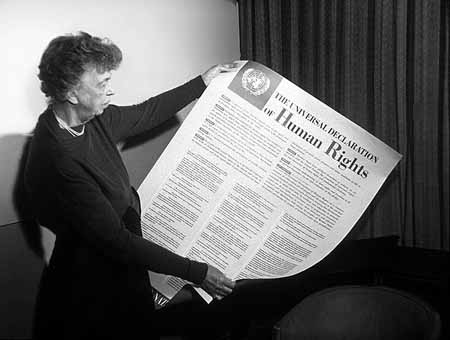
\includegraphics{images/Eleanor_Roosevelt_and_Human_Rights_Declaration.jpeg}
\caption{Eleanor Roosevelt hält die englische Version der Allgemeinen
Erklärung der Menschenrechte (FDR Presidential Library \& Museum, CC BY
2.0 \url{https://creativecommons.org/licenses/by/2.0}, via Wikimedia
Commons)}\label{fig:eleanor}
\end{figure}

All human beings are born free and equal in dignity and rights. All
human beings are born free and equal in dignity and rights. All human
beings are born free and equal in dignity and rights. All human beings
are born free and equal in dignity and rights.

\section{Code}\label{code}

All human beings are born free and equal in dignity and rights. All
human beings are born free and equal in dignity and rights. All human
beings are born free and equal in dignity and rights. All human beings
are born free and equal in dignity and rights.

\begin{Shaded}
\begin{Highlighting}[]
\FunctionTok{ping}\NormalTok{ wikipedia.org}
\end{Highlighting}
\end{Shaded}

All human beings are born free and equal in dignity and rights. All
human beings are born free and equal in dignity and rights. All human
beings are born free and equal in dignity and rights. All human beings
are born free and equal in dignity and rights.

\section{URLs and email addresses}\label{urls-and-email-addresses}

\href{https://www.wikipedia.org/}{wikipedia.org},
\href{mailto:info@wikipedia.org}{\nolinkurl{info@wikipedia.org}}. All
human beings are born free and equal in dignity and rights. All human
beings are born free and equal in dignity and rights. All human beings
are born free and equal in dignity and rights. All human beings are born
free and equal in dignity and rights.

\section{Tables}\label{tables}

\begin{longtable}[]{@{}
  >{\raggedright\arraybackslash}p{(\columnwidth - 2\tabcolsep) * \real{0.5000}}
  >{\raggedright\arraybackslash}p{(\columnwidth - 2\tabcolsep) * \real{0.5000}}@{}}
\caption{\label{tbl:example_tbl}Table caption}\tabularnewline
\toprule\noalign{}
\begin{minipage}[b]{\linewidth}\raggedright
column 1
\end{minipage} & \begin{minipage}[b]{\linewidth}\raggedright
column 2
\end{minipage} \\
\midrule\noalign{}
\endfirsthead
\toprule\noalign{}
\begin{minipage}[b]{\linewidth}\raggedright
column 1
\end{minipage} & \begin{minipage}[b]{\linewidth}\raggedright
column 2
\end{minipage} \\
\midrule\noalign{}
\endhead
\bottomrule\noalign{}
\endlastfoot
All human beings are born free and equal in dignity and rights. & All
human beings are born free and equal in dignity and rights. \\
All human beings are born free and equal in dignity and rights. & All
human beings are born free and equal in dignity and rights. \\
All human beings are born free and equal in dignity and rights. & All
human beings are born free and equal in dignity and rights. \\
All human beings are born free and equal in dignity and rights. & All
human beings are born free and equal in dignity and rights. \\
\end{longtable}

All human beings are born free and equal in dignity and rights. All
human beings are born free and equal in dignity and rights. All human
beings are born free and equal in dignity and rights. All human beings
are born free and equal in dignity and rights.

\section{Footnotes}\label{footnotes}

All human beings are born free and equal in dignity and rights. All
human beings are born free and equal in dignity and rights. All human
beings are born free and equal in dignity and rights. All human beings
are born free and equal in dignity and rights.\footnote{All human beings
  are born free and equal in dignity and rights.}

\section{Quotes}\label{quotes}

\begin{otherlanguage}{ngerman}

\begin{quote}
Alle Menschen sind frei und gleich an Würde und Rechten geboren.
\end{quote}

\end{otherlanguage}

All human beings are born free and equal in dignity and rights. All
human beings are born free and equal in dignity and rights. All human
beings are born free and equal in dignity and rights. All human beings
are born free and equal in dignity and rights.

\section{Scientific citations}\label{scientific-citations}

\begin{quote}
All human beings are born free and equal in dignity and rights. They are
endowed with reason and conscience and should act towards one another in
a spirit of brotherhood.Nations\footnote{\citeproc{ref-unitednations1948}{\emph{Universal
  {Declaration} of {Human} {Rights}}}.}
\end{quote}

All human beings are born free and equal in dignity and rights. All
human beings are born free and equal in dignity and rights. All human
beings are born free and equal in dignity and rights. All human beings
are born free and equal in dignity and rights.\footnote{\citeproc{ref-unitednations1948}{Nations}.}

\section{Equations}\label{equations}

\begin{equation}\phantomsection\label{eq:pythagoras}{x^2 + y^2 = z^2}\end{equation}

\section{Cross-references}\label{cross-references}

Thanks to
\href{https://lierdakil.github.io/pandoc-crossref/}{pandoc-crossref} you
can crossreference equations (eq.~\ref{eq:pythagoras}), figures
(Figure~\ref{fig:eleanor}) and tables (tbl.~\ref{tbl:example_tbl}).
Sections (sec.~\ref{sec:conclusion}) are not supported in LaTeX.

\chapter{Chapter 1}\label{sec:chapter1}

\section{A Universal Declaration of Human
Rights}\label{a-universal-declaration-of-human-rights}

\subsection{Preamble}\label{preamble}

Whereas recognition of the inherent dignity and of the equal and
inalienable rights of all members of the human family is the foundation
of freedom, justice and peace in the world,

Whereas disregard and contempt for human rights have resulted in
barbarous acts which have outraged the conscience of mankind, and the
advent of a world in which human beings shall enjoy freedom of speech
and belief and freedom from fear and want has been proclaimed as the
highest aspiration of the common people,

Whereas it is essential, if man is not to be compelled to have recourse,
as a last resort, to rebellion against tyranny and oppression, that
human rights should be protected by the rule of law,

Whereas it is essential to promote the development of friendly relations
between nations,

Whereas the peoples of the United Nations have in the Charter reaffirmed
their faith in fundamental human rights, in the dignity and worth of the
human person and in the equal rights of men and women and have
determined to promote social progress and better standards of life in
larger freedom,

Whereas Member States have pledged themselves to achieve, in
co-operation with the United Nations, the promotion of universal respect
for and observance of human rights and fundamental freedoms,

Whereas a common understanding of these rights and freedoms is of the
greatest importance for the full realization of this pledge,

Now, therefore,

The General Assembly

Proclaims this Universal Declaration of Human Rights as a common
standard of achievement for all peoples and all nations, to the end that
every individual and every organ of society, keeping this Declaration
constantly in mind, shall strive by teaching and education to promote
respect for these rights and freedoms and by progressive measures,
national and international, to secure their universal and effective
recognition and observance, both among the peoples of Member States
themselves and among the peoples of territories under their
jurisdiction.

\subsection{Article 1}\label{article-1}

All human beings are born free and equal in dignity and rights. They are
endowed with reason and conscience and should act towards one another in
a spirit of brotherhood.

\subsection{Article 2}\label{article-2}

Everyone is entitled to all the rights and freedoms set forth in this
Declaration, without distinction of any kind, such as race, colour, sex,
language, religion, political or other opinion, national or social
origin, property, birth or other status.

Furthermore, no distinction shall be made on the basis of the political,
jurisdictional or international status of the country or territory to
which a person belongs, whether it be independent, trust,
non-self-governing or under any other limitation of sovereignty.

\subsection{Article 3}\label{article-3}

Everyone has the right to life, liberty and the security of person.

\subsection{Article 4}\label{article-4}

No one shall be held in slavery or servitude; slavery and the slave
trade shall be prohibited in all their forms.

\subsection{Article 5}\label{article-5}

No one shall be subjected to torture or to cruel, inhuman or degrading
treatment or punishment.

\subsection{Article 6}\label{article-6}

Everyone has the right to recognition everywhere as a person before the
law.

\subsection{Article 7}\label{article-7}

All are equal before the law and are entitled without any discrimination
to equal protection of the law. All are entitled to equal protection
against any discrimination in violation of this Declaration and against
any incitement to such discrimination.

\subsection{Article 8}\label{article-8}

Everyone has the right to an effective remedy by the competent national
tribunals for acts violating the fundamental rights granted him by the
constitution or by law.

\subsection{Article 9}\label{article-9}

No one shall be subjected to arbitrary arrest, detention or exile.

\subsection{Article 10}\label{article-10}

Everyone is entitled in full equality to a fair and public hearing by an
independent and impartial tribunal, in the determination of his rights
and obligations and of any criminal charge against him.

\subsection{Article 11}\label{article-11}

\begin{enumerate}
\def\labelenumi{\arabic{enumi}.}
\item
  Everyone charged with a penal offence has the right to be presumed
  innocent until proved guilty according to law in a public trial at
  which he has had all the guarantees necessary for his defence.
\item
  No one shall be held guilty of any penal offence on account of any act
  or omission which did not constitute a penal offence, under national
  or international law, at the time when it was committed. Nor shall a
  heavier penalty be imposed than the one that was applicable at the
  time the penal offence was committed.
\end{enumerate}

\subsection{Article 12}\label{article-12}

No one shall be subjected to arbitrary interference with his privacy,
family, home or correspondence, nor to attacks upon his honour and
reputation. Everyone has the right to the protection of the law against
such interference or attacks.

\subsection{Article 13}\label{article-13}

\begin{enumerate}
\def\labelenumi{\arabic{enumi}.}
\item
  Everyone has the right to freedom of movement and residence within the
  borders of each State.
\item
  Everyone has the right to leave any country, including his own, and to
  return to his country.
\end{enumerate}

\subsection{Article 14}\label{article-14}

\begin{enumerate}
\def\labelenumi{\arabic{enumi}.}
\item
  Everyone has the right to seek and to enjoy in other countries asylum
  from persecution.
\item
  This right may not be invoked in the case of prosecutions genuinely
  arising from non-political crimes or from acts contrary to the
  purposes and principles of the United Nations.
\end{enumerate}

\subsection{Article 15}\label{article-15}

\begin{enumerate}
\def\labelenumi{\arabic{enumi}.}
\item
  Everyone has the right to a nationality.
\item
  No one shall be arbitrarily deprived of his nationality nor denied the
  right to change his nationality.
\end{enumerate}

\subsection{Article 16}\label{article-16}

\begin{enumerate}
\def\labelenumi{\arabic{enumi}.}
\item
  Men and women of full age, without any limitation due to race,
  nationality or religion, have the right to marry and to found a
  family. They are entitled to equal rights as to marriage, during
  marriage and at its dissolution.
\item
  Marriage shall be entered into only with the free and full consent of
  the intending spouses.
\item
  The family is the natural and fundamental group unit of society and is
  entitled to protection by society and the State.
\end{enumerate}

\subsection{Article 17}\label{article-17}

\begin{enumerate}
\def\labelenumi{\arabic{enumi}.}
\item
  Everyone has the right to own property alone as well as in association
  with others.
\item
  No one shall be arbitrarily deprived of his property.
\end{enumerate}

\subsection{Article 18}\label{article-18}

Everyone has the right to freedom of thought, conscience and religion;
this right includes freedom to change his religion or belief, and
freedom, either alone or in community with others and in public or
private, to manifest his religion or belief in teaching, practice,
worship and observance.

\subsection{Article 19}\label{article-19}

Everyone has the right to freedom of opinion and expression; this right
includes freedom to hold opinions without interference and to seek,
receive and impart information and ideas through any media and
regardless of frontiers.

\subsection{Article 20}\label{article-20}

\begin{enumerate}
\def\labelenumi{\arabic{enumi}.}
\item
  Everyone has the right to freedom of peaceful assembly and
  association.
\item
  No one may be compelled to belong to an association.
\end{enumerate}

\subsection{Article 21}\label{article-21}

\begin{enumerate}
\def\labelenumi{\arabic{enumi}.}
\item
  Everyone has the right to take part in the government of his country,
  directly or through freely chosen representatives.
\item
  Everyone has the right of equal access to public service in his
  country.
\item
  The will of the people shall be the basis of the authority of
  government; this will shall be expressed in periodic and genuine
  elections which shall be by universal and equal suffrage and shall be
  held by secret vote or by equivalent free voting procedures.
\end{enumerate}

\subsection{Article 22}\label{article-22}

Everyone, as a member of society, has the right to social security and
is entitled to realization, through national effort and international
co-operation and in accordance with the organization and resources of
each State, of the economic, social and cultural rights indispensable
for his dignity and the free development of his personality.

\subsection{Article 23}\label{article-23}

\begin{enumerate}
\def\labelenumi{\arabic{enumi}.}
\item
  Everyone has the right to work, to free choice of employment, to just
  and favourable conditions of work and to protection against
  unemployment.
\item
  Everyone, without any discrimination, has the right to equal pay for
  equal work.
\item
  Everyone who works has the right to just and favourable remuneration
  ensuring for himself and his family an existence worthy of human
  dignity, and supplemented, if necessary, by other means of social
  protection.
\item
  Everyone has the right to form and to join trade unions for the
  protection of his interests.
\end{enumerate}

\subsection{Article 24}\label{article-24}

Everyone has the right to rest and leisure, including reasonable
limitation of working hours and periodic holidays with pay.

\subsection{Article 25}\label{article-25}

\begin{enumerate}
\def\labelenumi{\arabic{enumi}.}
\item
  Everyone has the right to a standard of living adequate for the health
  and well-being of himself and of his family, including food, clothing,
  housing and medical care and necessary social services, and the right
  to security in the event of unemployment, sickness, disability,
  widowhood, old age or other lack of livelihood in circumstances beyond
  his control.
\item
  Motherhood and childhood are entitled to special care and assistance.
  All children, whether born in or out of wedlock, shall enjoy the same
  social protection.
\end{enumerate}

\subsection{Article 26}\label{article-26}

\begin{enumerate}
\def\labelenumi{\arabic{enumi}.}
\item
  Everyone has the right to education. Education shall be free, at least
  in the elementary and fundamental stages. Elementary education shall
  be compulsory. Technical and professional education shall be made
  generally available and higher education shall be equally accessible
  to all on the basis of merit.
\item
  Education shall be directed to the full development of the human
  personality and to the strengthening of respect for human rights and
  fundamental freedoms. It shall promote understanding, tolerance and
  friendship among all nations, racial or religious groups, and shall
  further the activities of the United Nations for the maintenance of
  peace.
\item
  Parents have a prior right to choose the kind of education that shall
  be given to their children.
\end{enumerate}

\subsection{Article 27}\label{article-27}

\begin{enumerate}
\def\labelenumi{\arabic{enumi}.}
\item
  Everyone has the right freely to participate in the cultural life of
  the community, to enjoy the arts and to share in scientific
  advancement and its benefits.
\item
  Everyone has the right to the protection of the moral and material
  interests resulting from any scientific, literary or artistic
  production of which he is the author.
\end{enumerate}

\subsection{Article 28}\label{article-28}

Everyone is entitled to a social and international order in which the
rights and freedoms set forth in this Declaration can be fully realized.

\subsection{Article 29}\label{article-29}

\begin{enumerate}
\def\labelenumi{\arabic{enumi}.}
\item
  Everyone has duties to the community in which alone the free and full
  development of his personality is possible.
\item
  In the exercise of his rights and freedoms, everyone shall be subject
  only to such limitations as are determined by law solely for the
  purpose of securing due recognition and respect for the rights and
  freedoms of others and of meeting the just requirements of morality,
  public order and the general welfare in a democratic society.
\item
  These rights and freedoms may in no case be exercised contrary to the
  purposes and principles of the United Nations.
\end{enumerate}

\subsection{Article 30}\label{article-30}

Nothing in this Declaration may be interpreted as implying for any
State, group or person any right to engage in any activity or to perform
any act aimed at the destruction of any of the rights and freedoms set
forth herein.

\chapter{Chapter 2}\label{sec:chapter2}

\section{A Universal Declaration of Human
Rights}\label{a-universal-declaration-of-human-rights-1}

\subsection{Preamble}\label{preamble-1}

Whereas recognition of the inherent dignity and of the equal and
inalienable rights of all members of the human family is the foundation
of freedom, justice and peace in the world,

Whereas disregard and contempt for human rights have resulted in
barbarous acts which have outraged the conscience of mankind, and the
advent of a world in which human beings shall enjoy freedom of speech
and belief and freedom from fear and want has been proclaimed as the
highest aspiration of the common people,

Whereas it is essential, if man is not to be compelled to have recourse,
as a last resort, to rebellion against tyranny and oppression, that
human rights should be protected by the rule of law,

Whereas it is essential to promote the development of friendly relations
between nations,

Whereas the peoples of the United Nations have in the Charter reaffirmed
their faith in fundamental human rights, in the dignity and worth of the
human person and in the equal rights of men and women and have
determined to promote social progress and better standards of life in
larger freedom,

Whereas Member States have pledged themselves to achieve, in
co-operation with the United Nations, the promotion of universal respect
for and observance of human rights and fundamental freedoms,

Whereas a common understanding of these rights and freedoms is of the
greatest importance for the full realization of this pledge,

Now, therefore,

The General Assembly

Proclaims this Universal Declaration of Human Rights as a common
standard of achievement for all peoples and all nations, to the end that
every individual and every organ of society, keeping this Declaration
constantly in mind, shall strive by teaching and education to promote
respect for these rights and freedoms and by progressive measures,
national and international, to secure their universal and effective
recognition and observance, both among the peoples of Member States
themselves and among the peoples of territories under their
jurisdiction.

\subsection{Article 1}\label{article-1-1}

All human beings are born free and equal in dignity and rights. They are
endowed with reason and conscience and should act towards one another in
a spirit of brotherhood.

\subsection{Article 2}\label{article-2-1}

Everyone is entitled to all the rights and freedoms set forth in this
Declaration, without distinction of any kind, such as race, colour, sex,
language, religion, political or other opinion, national or social
origin, property, birth or other status.

Furthermore, no distinction shall be made on the basis of the political,
jurisdictional or international status of the country or territory to
which a person belongs, whether it be independent, trust,
non-self-governing or under any other limitation of sovereignty.

\subsection{Article 3}\label{article-3-1}

Everyone has the right to life, liberty and the security of person.

\subsection{Article 4}\label{article-4-1}

No one shall be held in slavery or servitude; slavery and the slave
trade shall be prohibited in all their forms.

\subsection{Article 5}\label{article-5-1}

No one shall be subjected to torture or to cruel, inhuman or degrading
treatment or punishment.

\subsection{Article 6}\label{article-6-1}

Everyone has the right to recognition everywhere as a person before the
law.

\subsection{Article 7}\label{article-7-1}

All are equal before the law and are entitled without any discrimination
to equal protection of the law. All are entitled to equal protection
against any discrimination in violation of this Declaration and against
any incitement to such discrimination.

\subsection{Article 8}\label{article-8-1}

Everyone has the right to an effective remedy by the competent national
tribunals for acts violating the fundamental rights granted him by the
constitution or by law.

\subsection{Article 9}\label{article-9-1}

No one shall be subjected to arbitrary arrest, detention or exile.

\subsection{Article 10}\label{article-10-1}

Everyone is entitled in full equality to a fair and public hearing by an
independent and impartial tribunal, in the determination of his rights
and obligations and of any criminal charge against him.

\subsection{Article 11}\label{article-11-1}

\begin{enumerate}
\def\labelenumi{\arabic{enumi}.}
\item
  Everyone charged with a penal offence has the right to be presumed
  innocent until proved guilty according to law in a public trial at
  which he has had all the guarantees necessary for his defence.
\item
  No one shall be held guilty of any penal offence on account of any act
  or omission which did not constitute a penal offence, under national
  or international law, at the time when it was committed. Nor shall a
  heavier penalty be imposed than the one that was applicable at the
  time the penal offence was committed.
\end{enumerate}

\subsection{Article 12}\label{article-12-1}

No one shall be subjected to arbitrary interference with his privacy,
family, home or correspondence, nor to attacks upon his honour and
reputation. Everyone has the right to the protection of the law against
such interference or attacks.

\subsection{Article 13}\label{article-13-1}

\begin{enumerate}
\def\labelenumi{\arabic{enumi}.}
\item
  Everyone has the right to freedom of movement and residence within the
  borders of each State.
\item
  Everyone has the right to leave any country, including his own, and to
  return to his country.
\end{enumerate}

\subsection{Article 14}\label{article-14-1}

\begin{enumerate}
\def\labelenumi{\arabic{enumi}.}
\item
  Everyone has the right to seek and to enjoy in other countries asylum
  from persecution.
\item
  This right may not be invoked in the case of prosecutions genuinely
  arising from non-political crimes or from acts contrary to the
  purposes and principles of the United Nations.
\end{enumerate}

\subsection{Article 15}\label{article-15-1}

\begin{enumerate}
\def\labelenumi{\arabic{enumi}.}
\item
  Everyone has the right to a nationality.
\item
  No one shall be arbitrarily deprived of his nationality nor denied the
  right to change his nationality.
\end{enumerate}

\subsection{Article 16}\label{article-16-1}

\begin{enumerate}
\def\labelenumi{\arabic{enumi}.}
\item
  Men and women of full age, without any limitation due to race,
  nationality or religion, have the right to marry and to found a
  family. They are entitled to equal rights as to marriage, during
  marriage and at its dissolution.
\item
  Marriage shall be entered into only with the free and full consent of
  the intending spouses.
\item
  The family is the natural and fundamental group unit of society and is
  entitled to protection by society and the State.
\end{enumerate}

\subsection{Article 17}\label{article-17-1}

\begin{enumerate}
\def\labelenumi{\arabic{enumi}.}
\item
  Everyone has the right to own property alone as well as in association
  with others.
\item
  No one shall be arbitrarily deprived of his property.
\end{enumerate}

\subsection{Article 18}\label{article-18-1}

Everyone has the right to freedom of thought, conscience and religion;
this right includes freedom to change his religion or belief, and
freedom, either alone or in community with others and in public or
private, to manifest his religion or belief in teaching, practice,
worship and observance.

\subsection{Article 19}\label{article-19-1}

Everyone has the right to freedom of opinion and expression; this right
includes freedom to hold opinions without interference and to seek,
receive and impart information and ideas through any media and
regardless of frontiers.

\subsection{Article 20}\label{article-20-1}

\begin{enumerate}
\def\labelenumi{\arabic{enumi}.}
\item
  Everyone has the right to freedom of peaceful assembly and
  association.
\item
  No one may be compelled to belong to an association.
\end{enumerate}

\subsection{Article 21}\label{article-21-1}

\begin{enumerate}
\def\labelenumi{\arabic{enumi}.}
\item
  Everyone has the right to take part in the government of his country,
  directly or through freely chosen representatives.
\item
  Everyone has the right of equal access to public service in his
  country.
\item
  The will of the people shall be the basis of the authority of
  government; this will shall be expressed in periodic and genuine
  elections which shall be by universal and equal suffrage and shall be
  held by secret vote or by equivalent free voting procedures.
\end{enumerate}

\subsection{Article 22}\label{article-22-1}

Everyone, as a member of society, has the right to social security and
is entitled to realization, through national effort and international
co-operation and in accordance with the organization and resources of
each State, of the economic, social and cultural rights indispensable
for his dignity and the free development of his personality.

\subsection{Article 23}\label{article-23-1}

\begin{enumerate}
\def\labelenumi{\arabic{enumi}.}
\item
  Everyone has the right to work, to free choice of employment, to just
  and favourable conditions of work and to protection against
  unemployment.
\item
  Everyone, without any discrimination, has the right to equal pay for
  equal work.
\item
  Everyone who works has the right to just and favourable remuneration
  ensuring for himself and his family an existence worthy of human
  dignity, and supplemented, if necessary, by other means of social
  protection.
\item
  Everyone has the right to form and to join trade unions for the
  protection of his interests.
\end{enumerate}

\subsection{Article 24}\label{article-24-1}

Everyone has the right to rest and leisure, including reasonable
limitation of working hours and periodic holidays with pay.

\subsection{Article 25}\label{article-25-1}

\begin{enumerate}
\def\labelenumi{\arabic{enumi}.}
\item
  Everyone has the right to a standard of living adequate for the health
  and well-being of himself and of his family, including food, clothing,
  housing and medical care and necessary social services, and the right
  to security in the event of unemployment, sickness, disability,
  widowhood, old age or other lack of livelihood in circumstances beyond
  his control.
\item
  Motherhood and childhood are entitled to special care and assistance.
  All children, whether born in or out of wedlock, shall enjoy the same
  social protection.
\end{enumerate}

\subsection{Article 26}\label{article-26-1}

\begin{enumerate}
\def\labelenumi{\arabic{enumi}.}
\item
  Everyone has the right to education. Education shall be free, at least
  in the elementary and fundamental stages. Elementary education shall
  be compulsory. Technical and professional education shall be made
  generally available and higher education shall be equally accessible
  to all on the basis of merit.
\item
  Education shall be directed to the full development of the human
  personality and to the strengthening of respect for human rights and
  fundamental freedoms. It shall promote understanding, tolerance and
  friendship among all nations, racial or religious groups, and shall
  further the activities of the United Nations for the maintenance of
  peace.
\item
  Parents have a prior right to choose the kind of education that shall
  be given to their children.
\end{enumerate}

\subsection{Article 27}\label{article-27-1}

\begin{enumerate}
\def\labelenumi{\arabic{enumi}.}
\item
  Everyone has the right freely to participate in the cultural life of
  the community, to enjoy the arts and to share in scientific
  advancement and its benefits.
\item
  Everyone has the right to the protection of the moral and material
  interests resulting from any scientific, literary or artistic
  production of which he is the author.
\end{enumerate}

\subsection{Article 28}\label{article-28-1}

Everyone is entitled to a social and international order in which the
rights and freedoms set forth in this Declaration can be fully realized.

\subsection{Article 29}\label{article-29-1}

\begin{enumerate}
\def\labelenumi{\arabic{enumi}.}
\item
  Everyone has duties to the community in which alone the free and full
  development of his personality is possible.
\item
  In the exercise of his rights and freedoms, everyone shall be subject
  only to such limitations as are determined by law solely for the
  purpose of securing due recognition and respect for the rights and
  freedoms of others and of meeting the just requirements of morality,
  public order and the general welfare in a democratic society.
\item
  These rights and freedoms may in no case be exercised contrary to the
  purposes and principles of the United Nations.
\end{enumerate}

\subsection{Article 30}\label{article-30-1}

Nothing in this Declaration may be interpreted as implying for any
State, group or person any right to engage in any activity or to perform
any act aimed at the destruction of any of the rights and freedoms set
forth herein.

\chapter{Chapter 3}\label{sec:chapter3}

\section{A Universal Declaration of Human
Rights}\label{a-universal-declaration-of-human-rights-2}

\subsection{Preamble}\label{preamble-2}

Whereas recognition of the inherent dignity and of the equal and
inalienable rights of all members of the human family is the foundation
of freedom, justice and peace in the world,

Whereas disregard and contempt for human rights have resulted in
barbarous acts which have outraged the conscience of mankind, and the
advent of a world in which human beings shall enjoy freedom of speech
and belief and freedom from fear and want has been proclaimed as the
highest aspiration of the common people,

Whereas it is essential, if man is not to be compelled to have recourse,
as a last resort, to rebellion against tyranny and oppression, that
human rights should be protected by the rule of law,

Whereas it is essential to promote the development of friendly relations
between nations,

Whereas the peoples of the United Nations have in the Charter reaffirmed
their faith in fundamental human rights, in the dignity and worth of the
human person and in the equal rights of men and women and have
determined to promote social progress and better standards of life in
larger freedom,

Whereas Member States have pledged themselves to achieve, in
co-operation with the United Nations, the promotion of universal respect
for and observance of human rights and fundamental freedoms,

Whereas a common understanding of these rights and freedoms is of the
greatest importance for the full realization of this pledge,

Now, therefore,

The General Assembly

Proclaims this Universal Declaration of Human Rights as a common
standard of achievement for all peoples and all nations, to the end that
every individual and every organ of society, keeping this Declaration
constantly in mind, shall strive by teaching and education to promote
respect for these rights and freedoms and by progressive measures,
national and international, to secure their universal and effective
recognition and observance, both among the peoples of Member States
themselves and among the peoples of territories under their
jurisdiction.

\subsection{Article 1}\label{article-1-2}

All human beings are born free and equal in dignity and rights. They are
endowed with reason and conscience and should act towards one another in
a spirit of brotherhood.

\subsection{Article 2}\label{article-2-2}

Everyone is entitled to all the rights and freedoms set forth in this
Declaration, without distinction of any kind, such as race, colour, sex,
language, religion, political or other opinion, national or social
origin, property, birth or other status.

Furthermore, no distinction shall be made on the basis of the political,
jurisdictional or international status of the country or territory to
which a person belongs, whether it be independent, trust,
non-self-governing or under any other limitation of sovereignty.

\subsection{Article 3}\label{article-3-2}

Everyone has the right to life, liberty and the security of person.

\subsection{Article 4}\label{article-4-2}

No one shall be held in slavery or servitude; slavery and the slave
trade shall be prohibited in all their forms.

\subsection{Article 5}\label{article-5-2}

No one shall be subjected to torture or to cruel, inhuman or degrading
treatment or punishment.

\subsection{Article 6}\label{article-6-2}

Everyone has the right to recognition everywhere as a person before the
law.

\subsection{Article 7}\label{article-7-2}

All are equal before the law and are entitled without any discrimination
to equal protection of the law. All are entitled to equal protection
against any discrimination in violation of this Declaration and against
any incitement to such discrimination.

\subsection{Article 8}\label{article-8-2}

Everyone has the right to an effective remedy by the competent national
tribunals for acts violating the fundamental rights granted him by the
constitution or by law.

\subsection{Article 9}\label{article-9-2}

No one shall be subjected to arbitrary arrest, detention or exile.

\subsection{Article 10}\label{article-10-2}

Everyone is entitled in full equality to a fair and public hearing by an
independent and impartial tribunal, in the determination of his rights
and obligations and of any criminal charge against him.

\subsection{Article 11}\label{article-11-2}

\begin{enumerate}
\def\labelenumi{\arabic{enumi}.}
\item
  Everyone charged with a penal offence has the right to be presumed
  innocent until proved guilty according to law in a public trial at
  which he has had all the guarantees necessary for his defence.
\item
  No one shall be held guilty of any penal offence on account of any act
  or omission which did not constitute a penal offence, under national
  or international law, at the time when it was committed. Nor shall a
  heavier penalty be imposed than the one that was applicable at the
  time the penal offence was committed.
\end{enumerate}

\subsection{Article 12}\label{article-12-2}

No one shall be subjected to arbitrary interference with his privacy,
family, home or correspondence, nor to attacks upon his honour and
reputation. Everyone has the right to the protection of the law against
such interference or attacks.

\subsection{Article 13}\label{article-13-2}

\begin{enumerate}
\def\labelenumi{\arabic{enumi}.}
\item
  Everyone has the right to freedom of movement and residence within the
  borders of each State.
\item
  Everyone has the right to leave any country, including his own, and to
  return to his country.
\end{enumerate}

\subsection{Article 14}\label{article-14-2}

\begin{enumerate}
\def\labelenumi{\arabic{enumi}.}
\item
  Everyone has the right to seek and to enjoy in other countries asylum
  from persecution.
\item
  This right may not be invoked in the case of prosecutions genuinely
  arising from non-political crimes or from acts contrary to the
  purposes and principles of the United Nations.
\end{enumerate}

\subsection{Article 15}\label{article-15-2}

\begin{enumerate}
\def\labelenumi{\arabic{enumi}.}
\item
  Everyone has the right to a nationality.
\item
  No one shall be arbitrarily deprived of his nationality nor denied the
  right to change his nationality.
\end{enumerate}

\subsection{Article 16}\label{article-16-2}

\begin{enumerate}
\def\labelenumi{\arabic{enumi}.}
\item
  Men and women of full age, without any limitation due to race,
  nationality or religion, have the right to marry and to found a
  family. They are entitled to equal rights as to marriage, during
  marriage and at its dissolution.
\item
  Marriage shall be entered into only with the free and full consent of
  the intending spouses.
\item
  The family is the natural and fundamental group unit of society and is
  entitled to protection by society and the State.
\end{enumerate}

\subsection{Article 17}\label{article-17-2}

\begin{enumerate}
\def\labelenumi{\arabic{enumi}.}
\item
  Everyone has the right to own property alone as well as in association
  with others.
\item
  No one shall be arbitrarily deprived of his property.
\end{enumerate}

\subsection{Article 18}\label{article-18-2}

Everyone has the right to freedom of thought, conscience and religion;
this right includes freedom to change his religion or belief, and
freedom, either alone or in community with others and in public or
private, to manifest his religion or belief in teaching, practice,
worship and observance.

\subsection{Article 19}\label{article-19-2}

Everyone has the right to freedom of opinion and expression; this right
includes freedom to hold opinions without interference and to seek,
receive and impart information and ideas through any media and
regardless of frontiers.

\subsection{Article 20}\label{article-20-2}

\begin{enumerate}
\def\labelenumi{\arabic{enumi}.}
\item
  Everyone has the right to freedom of peaceful assembly and
  association.
\item
  No one may be compelled to belong to an association.
\end{enumerate}

\subsection{Article 21}\label{article-21-2}

\begin{enumerate}
\def\labelenumi{\arabic{enumi}.}
\item
  Everyone has the right to take part in the government of his country,
  directly or through freely chosen representatives.
\item
  Everyone has the right of equal access to public service in his
  country.
\item
  The will of the people shall be the basis of the authority of
  government; this will shall be expressed in periodic and genuine
  elections which shall be by universal and equal suffrage and shall be
  held by secret vote or by equivalent free voting procedures.
\end{enumerate}

\subsection{Article 22}\label{article-22-2}

Everyone, as a member of society, has the right to social security and
is entitled to realization, through national effort and international
co-operation and in accordance with the organization and resources of
each State, of the economic, social and cultural rights indispensable
for his dignity and the free development of his personality.

\subsection{Article 23}\label{article-23-2}

\begin{enumerate}
\def\labelenumi{\arabic{enumi}.}
\item
  Everyone has the right to work, to free choice of employment, to just
  and favourable conditions of work and to protection against
  unemployment.
\item
  Everyone, without any discrimination, has the right to equal pay for
  equal work.
\item
  Everyone who works has the right to just and favourable remuneration
  ensuring for himself and his family an existence worthy of human
  dignity, and supplemented, if necessary, by other means of social
  protection.
\item
  Everyone has the right to form and to join trade unions for the
  protection of his interests.
\end{enumerate}

\subsection{Article 24}\label{article-24-2}

Everyone has the right to rest and leisure, including reasonable
limitation of working hours and periodic holidays with pay.

\subsection{Article 25}\label{article-25-2}

\begin{enumerate}
\def\labelenumi{\arabic{enumi}.}
\item
  Everyone has the right to a standard of living adequate for the health
  and well-being of himself and of his family, including food, clothing,
  housing and medical care and necessary social services, and the right
  to security in the event of unemployment, sickness, disability,
  widowhood, old age or other lack of livelihood in circumstances beyond
  his control.
\item
  Motherhood and childhood are entitled to special care and assistance.
  All children, whether born in or out of wedlock, shall enjoy the same
  social protection.
\end{enumerate}

\subsection{Article 26}\label{article-26-2}

\begin{enumerate}
\def\labelenumi{\arabic{enumi}.}
\item
  Everyone has the right to education. Education shall be free, at least
  in the elementary and fundamental stages. Elementary education shall
  be compulsory. Technical and professional education shall be made
  generally available and higher education shall be equally accessible
  to all on the basis of merit.
\item
  Education shall be directed to the full development of the human
  personality and to the strengthening of respect for human rights and
  fundamental freedoms. It shall promote understanding, tolerance and
  friendship among all nations, racial or religious groups, and shall
  further the activities of the United Nations for the maintenance of
  peace.
\item
  Parents have a prior right to choose the kind of education that shall
  be given to their children.
\end{enumerate}

\subsection{Article 27}\label{article-27-2}

\begin{enumerate}
\def\labelenumi{\arabic{enumi}.}
\item
  Everyone has the right freely to participate in the cultural life of
  the community, to enjoy the arts and to share in scientific
  advancement and its benefits.
\item
  Everyone has the right to the protection of the moral and material
  interests resulting from any scientific, literary or artistic
  production of which he is the author.
\end{enumerate}

\subsection{Article 28}\label{article-28-2}

Everyone is entitled to a social and international order in which the
rights and freedoms set forth in this Declaration can be fully realized.

\subsection{Article 29}\label{article-29-2}

\begin{enumerate}
\def\labelenumi{\arabic{enumi}.}
\item
  Everyone has duties to the community in which alone the free and full
  development of his personality is possible.
\item
  In the exercise of his rights and freedoms, everyone shall be subject
  only to such limitations as are determined by law solely for the
  purpose of securing due recognition and respect for the rights and
  freedoms of others and of meeting the just requirements of morality,
  public order and the general welfare in a democratic society.
\item
  These rights and freedoms may in no case be exercised contrary to the
  purposes and principles of the United Nations.
\end{enumerate}

\subsection{Article 30}\label{article-30-2}

Nothing in this Declaration may be interpreted as implying for any
State, group or person any right to engage in any activity or to perform
any act aimed at the destruction of any of the rights and freedoms set
forth herein.

\chapter{Chapter 4}\label{sec:chapter4}

\section{A Universal Declaration of Human
Rights}\label{a-universal-declaration-of-human-rights-3}

\subsection{Preamble}\label{preamble-3}

Whereas recognition of the inherent dignity and of the equal and
inalienable rights of all members of the human family is the foundation
of freedom, justice and peace in the world,

Whereas disregard and contempt for human rights have resulted in
barbarous acts which have outraged the conscience of mankind, and the
advent of a world in which human beings shall enjoy freedom of speech
and belief and freedom from fear and want has been proclaimed as the
highest aspiration of the common people,

Whereas it is essential, if man is not to be compelled to have recourse,
as a last resort, to rebellion against tyranny and oppression, that
human rights should be protected by the rule of law,

Whereas it is essential to promote the development of friendly relations
between nations,

Whereas the peoples of the United Nations have in the Charter reaffirmed
their faith in fundamental human rights, in the dignity and worth of the
human person and in the equal rights of men and women and have
determined to promote social progress and better standards of life in
larger freedom,

Whereas Member States have pledged themselves to achieve, in
co-operation with the United Nations, the promotion of universal respect
for and observance of human rights and fundamental freedoms,

Whereas a common understanding of these rights and freedoms is of the
greatest importance for the full realization of this pledge,

Now, therefore,

The General Assembly

Proclaims this Universal Declaration of Human Rights as a common
standard of achievement for all peoples and all nations, to the end that
every individual and every organ of society, keeping this Declaration
constantly in mind, shall strive by teaching and education to promote
respect for these rights and freedoms and by progressive measures,
national and international, to secure their universal and effective
recognition and observance, both among the peoples of Member States
themselves and among the peoples of territories under their
jurisdiction.

\subsection{Article 1}\label{article-1-3}

All human beings are born free and equal in dignity and rights. They are
endowed with reason and conscience and should act towards one another in
a spirit of brotherhood.

\subsection{Article 2}\label{article-2-3}

Everyone is entitled to all the rights and freedoms set forth in this
Declaration, without distinction of any kind, such as race, colour, sex,
language, religion, political or other opinion, national or social
origin, property, birth or other status.

Furthermore, no distinction shall be made on the basis of the political,
jurisdictional or international status of the country or territory to
which a person belongs, whether it be independent, trust,
non-self-governing or under any other limitation of sovereignty.

\subsection{Article 3}\label{article-3-3}

Everyone has the right to life, liberty and the security of person.

\subsection{Article 4}\label{article-4-3}

No one shall be held in slavery or servitude; slavery and the slave
trade shall be prohibited in all their forms.

\subsection{Article 5}\label{article-5-3}

No one shall be subjected to torture or to cruel, inhuman or degrading
treatment or punishment.

\subsection{Article 6}\label{article-6-3}

Everyone has the right to recognition everywhere as a person before the
law.

\subsection{Article 7}\label{article-7-3}

All are equal before the law and are entitled without any discrimination
to equal protection of the law. All are entitled to equal protection
against any discrimination in violation of this Declaration and against
any incitement to such discrimination.

\subsection{Article 8}\label{article-8-3}

Everyone has the right to an effective remedy by the competent national
tribunals for acts violating the fundamental rights granted him by the
constitution or by law.

\subsection{Article 9}\label{article-9-3}

No one shall be subjected to arbitrary arrest, detention or exile.

\subsection{Article 10}\label{article-10-3}

Everyone is entitled in full equality to a fair and public hearing by an
independent and impartial tribunal, in the determination of his rights
and obligations and of any criminal charge against him.

\subsection{Article 11}\label{article-11-3}

\begin{enumerate}
\def\labelenumi{\arabic{enumi}.}
\item
  Everyone charged with a penal offence has the right to be presumed
  innocent until proved guilty according to law in a public trial at
  which he has had all the guarantees necessary for his defence.
\item
  No one shall be held guilty of any penal offence on account of any act
  or omission which did not constitute a penal offence, under national
  or international law, at the time when it was committed. Nor shall a
  heavier penalty be imposed than the one that was applicable at the
  time the penal offence was committed.
\end{enumerate}

\subsection{Article 12}\label{article-12-3}

No one shall be subjected to arbitrary interference with his privacy,
family, home or correspondence, nor to attacks upon his honour and
reputation. Everyone has the right to the protection of the law against
such interference or attacks.

\subsection{Article 13}\label{article-13-3}

\begin{enumerate}
\def\labelenumi{\arabic{enumi}.}
\item
  Everyone has the right to freedom of movement and residence within the
  borders of each State.
\item
  Everyone has the right to leave any country, including his own, and to
  return to his country.
\end{enumerate}

\subsection{Article 14}\label{article-14-3}

\begin{enumerate}
\def\labelenumi{\arabic{enumi}.}
\item
  Everyone has the right to seek and to enjoy in other countries asylum
  from persecution.
\item
  This right may not be invoked in the case of prosecutions genuinely
  arising from non-political crimes or from acts contrary to the
  purposes and principles of the United Nations.
\end{enumerate}

\subsection{Article 15}\label{article-15-3}

\begin{enumerate}
\def\labelenumi{\arabic{enumi}.}
\item
  Everyone has the right to a nationality.
\item
  No one shall be arbitrarily deprived of his nationality nor denied the
  right to change his nationality.
\end{enumerate}

\subsection{Article 16}\label{article-16-3}

\begin{enumerate}
\def\labelenumi{\arabic{enumi}.}
\item
  Men and women of full age, without any limitation due to race,
  nationality or religion, have the right to marry and to found a
  family. They are entitled to equal rights as to marriage, during
  marriage and at its dissolution.
\item
  Marriage shall be entered into only with the free and full consent of
  the intending spouses.
\item
  The family is the natural and fundamental group unit of society and is
  entitled to protection by society and the State.
\end{enumerate}

\subsection{Article 17}\label{article-17-3}

\begin{enumerate}
\def\labelenumi{\arabic{enumi}.}
\item
  Everyone has the right to own property alone as well as in association
  with others.
\item
  No one shall be arbitrarily deprived of his property.
\end{enumerate}

\subsection{Article 18}\label{article-18-3}

Everyone has the right to freedom of thought, conscience and religion;
this right includes freedom to change his religion or belief, and
freedom, either alone or in community with others and in public or
private, to manifest his religion or belief in teaching, practice,
worship and observance.

\subsection{Article 19}\label{article-19-3}

Everyone has the right to freedom of opinion and expression; this right
includes freedom to hold opinions without interference and to seek,
receive and impart information and ideas through any media and
regardless of frontiers.

\subsection{Article 20}\label{article-20-3}

\begin{enumerate}
\def\labelenumi{\arabic{enumi}.}
\item
  Everyone has the right to freedom of peaceful assembly and
  association.
\item
  No one may be compelled to belong to an association.
\end{enumerate}

\subsection{Article 21}\label{article-21-3}

\begin{enumerate}
\def\labelenumi{\arabic{enumi}.}
\item
  Everyone has the right to take part in the government of his country,
  directly or through freely chosen representatives.
\item
  Everyone has the right of equal access to public service in his
  country.
\item
  The will of the people shall be the basis of the authority of
  government; this will shall be expressed in periodic and genuine
  elections which shall be by universal and equal suffrage and shall be
  held by secret vote or by equivalent free voting procedures.
\end{enumerate}

\subsection{Article 22}\label{article-22-3}

Everyone, as a member of society, has the right to social security and
is entitled to realization, through national effort and international
co-operation and in accordance with the organization and resources of
each State, of the economic, social and cultural rights indispensable
for his dignity and the free development of his personality.

\subsection{Article 23}\label{article-23-3}

\begin{enumerate}
\def\labelenumi{\arabic{enumi}.}
\item
  Everyone has the right to work, to free choice of employment, to just
  and favourable conditions of work and to protection against
  unemployment.
\item
  Everyone, without any discrimination, has the right to equal pay for
  equal work.
\item
  Everyone who works has the right to just and favourable remuneration
  ensuring for himself and his family an existence worthy of human
  dignity, and supplemented, if necessary, by other means of social
  protection.
\item
  Everyone has the right to form and to join trade unions for the
  protection of his interests.
\end{enumerate}

\subsection{Article 24}\label{article-24-3}

Everyone has the right to rest and leisure, including reasonable
limitation of working hours and periodic holidays with pay.

\subsection{Article 25}\label{article-25-3}

\begin{enumerate}
\def\labelenumi{\arabic{enumi}.}
\item
  Everyone has the right to a standard of living adequate for the health
  and well-being of himself and of his family, including food, clothing,
  housing and medical care and necessary social services, and the right
  to security in the event of unemployment, sickness, disability,
  widowhood, old age or other lack of livelihood in circumstances beyond
  his control.
\item
  Motherhood and childhood are entitled to special care and assistance.
  All children, whether born in or out of wedlock, shall enjoy the same
  social protection.
\end{enumerate}

\subsection{Article 26}\label{article-26-3}

\begin{enumerate}
\def\labelenumi{\arabic{enumi}.}
\item
  Everyone has the right to education. Education shall be free, at least
  in the elementary and fundamental stages. Elementary education shall
  be compulsory. Technical and professional education shall be made
  generally available and higher education shall be equally accessible
  to all on the basis of merit.
\item
  Education shall be directed to the full development of the human
  personality and to the strengthening of respect for human rights and
  fundamental freedoms. It shall promote understanding, tolerance and
  friendship among all nations, racial or religious groups, and shall
  further the activities of the United Nations for the maintenance of
  peace.
\item
  Parents have a prior right to choose the kind of education that shall
  be given to their children.
\end{enumerate}

\subsection{Article 27}\label{article-27-3}

\begin{enumerate}
\def\labelenumi{\arabic{enumi}.}
\item
  Everyone has the right freely to participate in the cultural life of
  the community, to enjoy the arts and to share in scientific
  advancement and its benefits.
\item
  Everyone has the right to the protection of the moral and material
  interests resulting from any scientific, literary or artistic
  production of which he is the author.
\end{enumerate}

\subsection{Article 28}\label{article-28-3}

Everyone is entitled to a social and international order in which the
rights and freedoms set forth in this Declaration can be fully realized.

\subsection{Article 29}\label{article-29-3}

\begin{enumerate}
\def\labelenumi{\arabic{enumi}.}
\item
  Everyone has duties to the community in which alone the free and full
  development of his personality is possible.
\item
  In the exercise of his rights and freedoms, everyone shall be subject
  only to such limitations as are determined by law solely for the
  purpose of securing due recognition and respect for the rights and
  freedoms of others and of meeting the just requirements of morality,
  public order and the general welfare in a democratic society.
\item
  These rights and freedoms may in no case be exercised contrary to the
  purposes and principles of the United Nations.
\end{enumerate}

\subsection{Article 30}\label{article-30-3}

Nothing in this Declaration may be interpreted as implying for any
State, group or person any right to engage in any activity or to perform
any act aimed at the destruction of any of the rights and freedoms set
forth herein.

\chapter{Conclusion}\label{sec:conclusion}

\section{A Universal Declaration of Human
Rights}\label{a-universal-declaration-of-human-rights-4}

\subsection{Preamble}\label{preamble-4}

Whereas recognition of the inherent dignity and of the equal and
inalienable rights of all members of the human family is the foundation
of freedom, justice and peace in the world,

Whereas disregard and contempt for human rights have resulted in
barbarous acts which have outraged the conscience of mankind, and the
advent of a world in which human beings shall enjoy freedom of speech
and belief and freedom from fear and want has been proclaimed as the
highest aspiration of the common people,

Whereas it is essential, if man is not to be compelled to have recourse,
as a last resort, to rebellion against tyranny and oppression, that
human rights should be protected by the rule of law,

Whereas it is essential to promote the development of friendly relations
between nations,

Whereas the peoples of the United Nations have in the Charter reaffirmed
their faith in fundamental human rights, in the dignity and worth of the
human person and in the equal rights of men and women and have
determined to promote social progress and better standards of life in
larger freedom,

Whereas Member States have pledged themselves to achieve, in
co-operation with the United Nations, the promotion of universal respect
for and observance of human rights and fundamental freedoms,

Whereas a common understanding of these rights and freedoms is of the
greatest importance for the full realization of this pledge,

Now, therefore,

The General Assembly

Proclaims this Universal Declaration of Human Rights as a common
standard of achievement for all peoples and all nations, to the end that
every individual and every organ of society, keeping this Declaration
constantly in mind, shall strive by teaching and education to promote
respect for these rights and freedoms and by progressive measures,
national and international, to secure their universal and effective
recognition and observance, both among the peoples of Member States
themselves and among the peoples of territories under their
jurisdiction.

\subsection{Article 1}\label{article-1-4}

All human beings are born free and equal in dignity and rights. They are
endowed with reason and conscience and should act towards one another in
a spirit of brotherhood.

\subsection{Article 2}\label{article-2-4}

Everyone is entitled to all the rights and freedoms set forth in this
Declaration, without distinction of any kind, such as race, colour, sex,
language, religion, political or other opinion, national or social
origin, property, birth or other status.

Furthermore, no distinction shall be made on the basis of the political,
jurisdictional or international status of the country or territory to
which a person belongs, whether it be independent, trust,
non-self-governing or under any other limitation of sovereignty.

\subsection{Article 3}\label{article-3-4}

Everyone has the right to life, liberty and the security of person.

\subsection{Article 4}\label{article-4-4}

No one shall be held in slavery or servitude; slavery and the slave
trade shall be prohibited in all their forms.

\subsection{Article 5}\label{article-5-4}

No one shall be subjected to torture or to cruel, inhuman or degrading
treatment or punishment.

\subsection{Article 6}\label{article-6-4}

Everyone has the right to recognition everywhere as a person before the
law.

\subsection{Article 7}\label{article-7-4}

All are equal before the law and are entitled without any discrimination
to equal protection of the law. All are entitled to equal protection
against any discrimination in violation of this Declaration and against
any incitement to such discrimination.

\subsection{Article 8}\label{article-8-4}

Everyone has the right to an effective remedy by the competent national
tribunals for acts violating the fundamental rights granted him by the
constitution or by law.

\subsection{Article 9}\label{article-9-4}

No one shall be subjected to arbitrary arrest, detention or exile.

\subsection{Article 10}\label{article-10-4}

Everyone is entitled in full equality to a fair and public hearing by an
independent and impartial tribunal, in the determination of his rights
and obligations and of any criminal charge against him.

\subsection{Article 11}\label{article-11-4}

\begin{enumerate}
\def\labelenumi{\arabic{enumi}.}
\item
  Everyone charged with a penal offence has the right to be presumed
  innocent until proved guilty according to law in a public trial at
  which he has had all the guarantees necessary for his defence.
\item
  No one shall be held guilty of any penal offence on account of any act
  or omission which did not constitute a penal offence, under national
  or international law, at the time when it was committed. Nor shall a
  heavier penalty be imposed than the one that was applicable at the
  time the penal offence was committed.
\end{enumerate}

\subsection{Article 12}\label{article-12-4}

No one shall be subjected to arbitrary interference with his privacy,
family, home or correspondence, nor to attacks upon his honour and
reputation. Everyone has the right to the protection of the law against
such interference or attacks.

\subsection{Article 13}\label{article-13-4}

\begin{enumerate}
\def\labelenumi{\arabic{enumi}.}
\item
  Everyone has the right to freedom of movement and residence within the
  borders of each State.
\item
  Everyone has the right to leave any country, including his own, and to
  return to his country.
\end{enumerate}

\subsection{Article 14}\label{article-14-4}

\begin{enumerate}
\def\labelenumi{\arabic{enumi}.}
\item
  Everyone has the right to seek and to enjoy in other countries asylum
  from persecution.
\item
  This right may not be invoked in the case of prosecutions genuinely
  arising from non-political crimes or from acts contrary to the
  purposes and principles of the United Nations.
\end{enumerate}

\subsection{Article 15}\label{article-15-4}

\begin{enumerate}
\def\labelenumi{\arabic{enumi}.}
\item
  Everyone has the right to a nationality.
\item
  No one shall be arbitrarily deprived of his nationality nor denied the
  right to change his nationality.
\end{enumerate}

\subsection{Article 16}\label{article-16-4}

\begin{enumerate}
\def\labelenumi{\arabic{enumi}.}
\item
  Men and women of full age, without any limitation due to race,
  nationality or religion, have the right to marry and to found a
  family. They are entitled to equal rights as to marriage, during
  marriage and at its dissolution.
\item
  Marriage shall be entered into only with the free and full consent of
  the intending spouses.
\item
  The family is the natural and fundamental group unit of society and is
  entitled to protection by society and the State.
\end{enumerate}

\subsection{Article 17}\label{article-17-4}

\begin{enumerate}
\def\labelenumi{\arabic{enumi}.}
\item
  Everyone has the right to own property alone as well as in association
  with others.
\item
  No one shall be arbitrarily deprived of his property.
\end{enumerate}

\subsection{Article 18}\label{article-18-4}

Everyone has the right to freedom of thought, conscience and religion;
this right includes freedom to change his religion or belief, and
freedom, either alone or in community with others and in public or
private, to manifest his religion or belief in teaching, practice,
worship and observance.

\subsection{Article 19}\label{article-19-4}

Everyone has the right to freedom of opinion and expression; this right
includes freedom to hold opinions without interference and to seek,
receive and impart information and ideas through any media and
regardless of frontiers.

\subsection{Article 20}\label{article-20-4}

\begin{enumerate}
\def\labelenumi{\arabic{enumi}.}
\item
  Everyone has the right to freedom of peaceful assembly and
  association.
\item
  No one may be compelled to belong to an association.
\end{enumerate}

\subsection{Article 21}\label{article-21-4}

\begin{enumerate}
\def\labelenumi{\arabic{enumi}.}
\item
  Everyone has the right to take part in the government of his country,
  directly or through freely chosen representatives.
\item
  Everyone has the right of equal access to public service in his
  country.
\item
  The will of the people shall be the basis of the authority of
  government; this will shall be expressed in periodic and genuine
  elections which shall be by universal and equal suffrage and shall be
  held by secret vote or by equivalent free voting procedures.
\end{enumerate}

\subsection{Article 22}\label{article-22-4}

Everyone, as a member of society, has the right to social security and
is entitled to realization, through national effort and international
co-operation and in accordance with the organization and resources of
each State, of the economic, social and cultural rights indispensable
for his dignity and the free development of his personality.

\subsection{Article 23}\label{article-23-4}

\begin{enumerate}
\def\labelenumi{\arabic{enumi}.}
\item
  Everyone has the right to work, to free choice of employment, to just
  and favourable conditions of work and to protection against
  unemployment.
\item
  Everyone, without any discrimination, has the right to equal pay for
  equal work.
\item
  Everyone who works has the right to just and favourable remuneration
  ensuring for himself and his family an existence worthy of human
  dignity, and supplemented, if necessary, by other means of social
  protection.
\item
  Everyone has the right to form and to join trade unions for the
  protection of his interests.
\end{enumerate}

\subsection{Article 24}\label{article-24-4}

Everyone has the right to rest and leisure, including reasonable
limitation of working hours and periodic holidays with pay.

\subsection{Article 25}\label{article-25-4}

\begin{enumerate}
\def\labelenumi{\arabic{enumi}.}
\item
  Everyone has the right to a standard of living adequate for the health
  and well-being of himself and of his family, including food, clothing,
  housing and medical care and necessary social services, and the right
  to security in the event of unemployment, sickness, disability,
  widowhood, old age or other lack of livelihood in circumstances beyond
  his control.
\item
  Motherhood and childhood are entitled to special care and assistance.
  All children, whether born in or out of wedlock, shall enjoy the same
  social protection.
\end{enumerate}

\subsection{Article 26}\label{article-26-4}

\begin{enumerate}
\def\labelenumi{\arabic{enumi}.}
\item
  Everyone has the right to education. Education shall be free, at least
  in the elementary and fundamental stages. Elementary education shall
  be compulsory. Technical and professional education shall be made
  generally available and higher education shall be equally accessible
  to all on the basis of merit.
\item
  Education shall be directed to the full development of the human
  personality and to the strengthening of respect for human rights and
  fundamental freedoms. It shall promote understanding, tolerance and
  friendship among all nations, racial or religious groups, and shall
  further the activities of the United Nations for the maintenance of
  peace.
\item
  Parents have a prior right to choose the kind of education that shall
  be given to their children.
\end{enumerate}

\subsection{Article 27}\label{article-27-4}

\begin{enumerate}
\def\labelenumi{\arabic{enumi}.}
\item
  Everyone has the right freely to participate in the cultural life of
  the community, to enjoy the arts and to share in scientific
  advancement and its benefits.
\item
  Everyone has the right to the protection of the moral and material
  interests resulting from any scientific, literary or artistic
  production of which he is the author.
\end{enumerate}

\subsection{Article 28}\label{article-28-4}

Everyone is entitled to a social and international order in which the
rights and freedoms set forth in this Declaration can be fully realized.

\subsection{Article 29}\label{article-29-4}

\begin{enumerate}
\def\labelenumi{\arabic{enumi}.}
\item
  Everyone has duties to the community in which alone the free and full
  development of his personality is possible.
\item
  In the exercise of his rights and freedoms, everyone shall be subject
  only to such limitations as are determined by law solely for the
  purpose of securing due recognition and respect for the rights and
  freedoms of others and of meeting the just requirements of morality,
  public order and the general welfare in a democratic society.
\item
  These rights and freedoms may in no case be exercised contrary to the
  purposes and principles of the United Nations.
\end{enumerate}

\subsection{Article 30}\label{article-30-4}

Nothing in this Declaration may be interpreted as implying for any
State, group or person any right to engage in any activity or to perform
any act aimed at the destruction of any of the rights and freedoms set
forth herein.

\chapter{Acknowledgment}\label{sec:acknowledgment}

Whereas recognition of the inherent dignity and of the equal and
inalienable rights of all members of the human family is the foundation
of freedom, justice and peace in the world,

Whereas disregard and contempt for human rights have resulted in
barbarous acts which have outraged the conscience of mankind, and the
advent of a world in which human beings shall enjoy freedom of speech
and belief and freedom from fear and want has been proclaimed as the
highest aspiration of the common people,

Whereas it is essential, if man is not to be compelled to have recourse,
as a last resort, to rebellion against tyranny and oppression, that
human rights should be protected by the rule of law,

Whereas it is essential to promote the development of friendly relations
between nations,

Whereas the peoples of the United Nations have in the Charter reaffirmed
their faith in fundamental human rights, in the dignity and worth of the
human person and in the equal rights of men and women and have
determined to promote social progress and better standards of life in
larger freedom,

Whereas Member States have pledged themselves to achieve, in
co-operation with the United Nations, the promotion of universal respect
for and observance of human rights and fundamental freedoms,

Whereas a common understanding of these rights and freedoms is of the
greatest importance for the full realization of this pledge,

Now, therefore,

The General Assembly

Proclaims this Universal Declaration of Human Rights as a common
standard of achievement for all peoples and all nations, to the end that
every individual and every organ of society, keeping this Declaration
constantly in mind, shall strive by teaching and education to promote
respect for these rights and freedoms and by progressive measures,
national and international, to secure their universal and effective
recognition and observance, both among the peoples of Member States
themselves and among the peoples of territories under their
jurisdiction.

%FIXME custom line spacing for appendix
\setstretch{1}

\listoffigures

\chapter{Bibliography}\label{bibliography}

\section{Sources}\label{sources}

\phantomsection\label{refs_sources}
\begin{CSLReferences}{1}{0}
\bibitem[\citeproctext]{ref-unitednations1948}
Nations, United. \emph{Universal {Declaration} of {Human} {Rights}},
1948.

\end{CSLReferences}

\clearpage

\section{Literature}\label{literature}

\phantomsection\label{refs_main}
\begin{CSLReferences}{1}{0}
\bibitem[\citeproctext]{ref-brown2016}
Brown, Gordon, ed. \emph{The {Universal} {Declaration} of {Human}
{Rights} in the 21st Century, a Living Document in a Changing World}.
Cambridge, {[}New York{]}: Open Book Publishers ; NYU Global Institute
for Advanced Study, 2016.

\end{CSLReferences}

\backmatter


\end{document}
